\usetikzlibrary{arrows.meta}
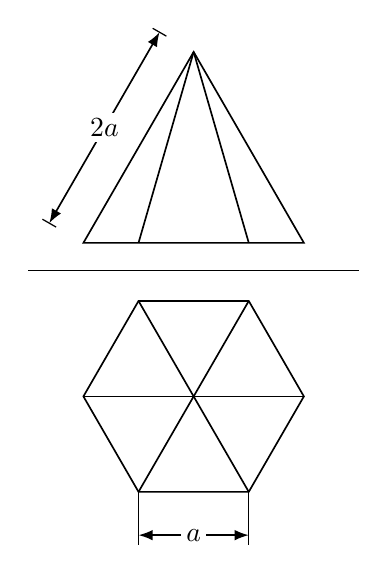
\begin{tikzpicture}[line width=.6pt,font=\normalsize,x=1cm,y=1cm]
\coordinate (S) at (0,2.425);
\coordinate (L) at (-1.4,0);
\coordinate (R) at (1.4,0);
\coordinate (Li) at (-0.7,0);
\coordinate (Ri) at (0.7,0);
\coordinate (E1) at (-1.833,0.25);
\coordinate (E2) at (-0.433,2.675);
\coordinate (H0) at (1.4,-1.95);
\coordinate (H1) at (0.7,-0.738);
\coordinate (H2) at (-0.7,-0.738);
\coordinate (H3) at (-1.4,-1.95);
\coordinate (H4) at (-0.7,-3.162);
\coordinate (H5) at (0.7,-3.162);
% front view
\draw (L) -- (S) -- (R) -- cycle;
\draw (S) -- (Li);
\draw (S) -- (Ri);
% 2a dimension along the left lateral edge
\draw[{Latex[length=1.8mm]}-{Latex[length=1.8mm]}] (E1) -- node[fill=white, inner sep=2pt] {$2a$} (E2);
\draw[line width=.45pt] (-1.92,0.3) -- (-1.746,0.2);
\draw[line width=.45pt] (-0.52,2.725) -- (-0.346,2.625);
% ground line
\draw[line width=.45pt] (-2.1,-0.35) -- (2.1,-0.35);
% plan view: regular hexagon with the three long diagonals
\draw (H0) -- (H1) -- (H2) -- (H3) -- (H4) -- (H5) -- cycle;
\draw (H0) -- (H3);
\draw (H1) -- (H4);
\draw (H2) -- (H5);
% a dimension under the bottom side
\draw[line width=.45pt] (H4) -- (-0.7,-3.832);
\draw[line width=.45pt] (H5) -- (0.7,-3.832);
\draw[{Latex[length=1.8mm]}-{Latex[length=1.8mm]}] (-0.7,-3.712) -- node[fill=white, inner sep=2pt] {$a$} (0.7,-3.712);
\end{tikzpicture}
